\chapter{美しいスクリーンショットを貼り付ける方法}
\label{chap:screenshot}

\LaTeX で文書を作る際の難しさの一つに、スクリーンショットの処理があります。

この文書では、\LaTeX 文書に美しくスクリーンショットを張り付ける方法を説明します。
なお、スクリーンショットを撮るOSはWindows11を想定しています。

\section{スクリーンショットは何故汚いか}

\begin{wrapfigure}[11]{r}[0pt]{0.5\textwidth}
  \begin{center}
    \includegraphics*[width=50mm]{image/sc100.pdf}
    \caption{通常のスクリーンショット} \label{fig:normal_ss}
  \end{center}
\end{wrapfigure}

まずは図\ref{fig:normal_ss}を見てください。

お世辞にもきれいとは言えないスクリーンショットです。このスクリーンショットはWindows上で
ごく普通の方法で取得したものを張り付けています。このスクリーンショットを撮ったときには、Windowsの
画面表示はここまでひどいものではありませんでした。

こうまでひどくなったのには理由があります。Windowsで撮ったスクリーンショットは、\LaTeX 文書に
張り付けてPDFに変換する際、紙面サイズや\LaTeX 図形表示サイズに合わせてスケーリングされます。
この際、なるべくきれいにスケーリングするアルゴリズムが選ばれてはいるものの、もともとの図形が細かい
ため、どうしても細部が崩れてしまうのです。

では次に図\ref{fig:beautiful_ss}を見てください。図\ref{fig:normal_ss}に比べて
格段に美しいスクリーンショットです。拡大すれば粗が見えるものの、画面で見るPDFの品質としては
十分ではないでしょうか。

図\ref{fig:beautiful_ss}が美しい秘密は、その大きさにあります。実は、このスクリーンショットは
図\ref{fig:normal_ss}の倍のサイズで表示されたものを取得しているのです。つまり、長さ方向で
倍の情報を持っているため、スケーリングするときに有利になるわけです。

\begin{wrapfigure}[11]{r}[0pt]{0.5\textwidth}
  \begin{center}
    \includegraphics*[width=50mm]{image/sc200.pdf}
    \caption{200\%拡大スクリーンショット} \label{fig:beautiful_ss}
  \end{center}
\end{wrapfigure}



この例では200\%拡大のスクリーンショットですが、400\%拡大でスクリーンショットを撮れば
印刷にも耐える品質になります。というわけで、大きなスクリーンショットをどうやって撮るか
知ることこそが、美しいスクリーンショットを\LaTeX 文書に張り付ける秘訣なのです。

この文書では、\LaTeX 文書に張り付けるための大きなスクリーンショットの撮り方を説明します。

\section{大きなスクリーンショットの撮り方}
大きなスクリーンショットを撮る理屈は簡単です。画面拡大率を大きくしてスクリーンショットを
撮ればよいのです。

\begin{figure}[bp]
  \begin{center}
    \includegraphics*[width=85mm]{image/system-display.pdf}
    \caption{Windowsの拡大縮小設定} \label{fig:system-display}
  \end{center}
\end{figure}

図\ref{fig:system-display}に、Windows11の拡大縮小設定画面を示します。
この設定画面は、コントロールパネルの中の、システム / ディスプレイを開くことで
見ることができます。

このスクリーンショットによれば、設定は200\%となっています。つまり、絵や文字は
我々に見やすいサイズの200\%で表示されているのです。このため、スクリーンショットは
倍のサイズで取得することができ、きれいに貼りつけることができるわけです。

しかしながら、狭い画面に倍のサイズで表示すると非常に作業性が悪くなります。

そこで、続く節ではあの手この手でこの「倍のサイズのスクリーンショット」を
作業性を落とさずに取得する方法を説明します。

どの手法もカギになるのはフレームバッファのサイズです。フレームバッファはコンピュータが
ディスプレイに写すための最終的な画面の情報を保持するバッファです。ここにある絵が
そのままディスプレイに表示されていると普通は考えられます。
また、このバッファを
ファイルに保存することでスクリーンショットを取得することができます。
つまり、フレームバッファの
サイズを大きくすることができれば、大きなスクリーンショットを撮ることができます。


一方で、現代の
コンピュータは複雑です。必ずしも物事が単純に進むとは限りません。
そこでその複雑さを逆手にとって、なるべく手軽に大きなスクリーンショットを
撮る方法がこの文書で紹介する数々の手法です。

\subsection{4Kディスプレイを使う}
大きなスクリーンショットをとる一番簡単な方法は、4kディスプレイを使うことです。

4kディスプレイを接続すれば、Windows PC内部のフレームバッファも自動的に4kサイズに
なります。この様子を図\ref{fig:4k-display}に示します。4kディスプレイの表示エリアは広大です
ので、Windowsの拡大縮小設定を200\%相当にしてもなお2kディスプレイ相当の情報を
表示することができます。

\begin{figure}[btp]
  \begin{center}
    \includegraphics*[width=70mm]{image/4kdisplay.pdf}
    \caption{4kディスプレイを使う} \label{fig:4k-display}
  \end{center}
\end{figure}

少々もったいない方法ですが、スクリーンショットを撮るときだけ我慢すればよいことですし、
作業性もそれほど低下しません。

4kディスプレイの価格もだいぶこなれてきましたので、4kディスプレイを使うことのできる人は
この方法を使うとよいでしょう。

\subsection{GPUを使う}
4kディスプレイを使わずとも、GPUを使うと内部で4kサイズのフレームバッファを作ることができます。

例えばAMDのRadeon GPUシリーズは、VSR (Virtual Super Resolution)と呼ばれるダウンスケーリング
機能を持っています。これはもともとゲーム用のもので、Windows内部のフレームバッファに大きくレンダリング
しておき、GPUで縮小してディスプレイに表示することでゲームの画面品質を上げようというものです。

この機能はOSのフレームバッファを入力として扱いますので、ゲームに限らず普通のアプリケーションにも
縮小が適用されます。そこでこの大きなフレームバッファからスクリーンショットを撮れば
目的を達成することができます。

具体的には、図\ref{fig:gpu}に表したように、外部の2kディスプレイに対して内部で4kフレームバッファを
用意するといった構成をとります。

\begin{figure}[btp]
  \begin{center}
    \includegraphics*[width=70mm]{image/gpu.pdf}
    \caption{GPUを使う} \label{fig:gpu}
  \end{center}
\end{figure}

AMDのRadeonシリーズの場合は、設定手順は次のようになります。


\begin{enumerate}
  \item AMDのAdrenaline Editionツールで、「仮想解像度」機能を有効にする。
  \item Windowsのディスプレイ設定の解像度の選択肢が増えるので、4kなどの大きな解像度を選ぶ。
  \item Windowsのディスプレイ設定の拡大率を200\%にする。
\end{enumerate}

モニタへの出力解像度は指定できませんが、それはAMDのツールが一番良い解像度を設定してくれます。


AMDのVSRはRadeon RX6400のようなローエンドのGPUやRyzen 5 2600GのようなAPUにも
搭載されています。調べた限りでは2024年3月時点で生産されているAMDの全GPU製品
(APU内蔵GPUを含む)でこの機能を使うことができるはずです。ただし、ほとんどの場合スペックに明記
されていないので買う前に調べることをお勧めします。

AMD以外に目を向けてみると、NVIDIAのGPUにはAMDのVSRに相当するDSR技術がありますので同様の設定が使えるはずです。

一方でIntelのGPU製品(APU内蔵GPUを含む)は、この機能に対応していません。
また、詳細不明ですが内蔵GPU付きのIntel CPUにNVIDIAのGPUを組み合わせた
ノートPCでは、この方法を使えないという情報もあります。

GPUによる縮小は非常に手軽でレスポンスも良く、8kといった解像度のフレームバッファも気軽に使えますのでお勧めできる方法です。

\subsection{仮想マシンを使う}
VMWare WorkstationやVirtualBoxといった仮想化ソフトを使うと、
PCに接続しているディスプレイよりも画面サイズの大きな仮想ディスプレイを
作ることができます。

\begin{figure}[btp]
  \begin{center}
    \includegraphics*[width=100mm]{image/vmware.pdf}
    \caption{仮想マシンを使う} \label{fig:vm}
  \end{center}
\end{figure}


この仮想ディスプレイは、直接物理ディスプレイには出力されず、あくまで
アプリケーションのフレームバッファとして扱われます(図\ref{fig:vm})。そして、ホストOSの
フレームバッファにコピーされる際、縮小されます。

この機能を使うことによって、4k仮想ディスプレイへの表示を縮小して
2kディスプレイで見ながら作業する事ができます。

この方法は外部にハードウェアを必要としませんが、仮想マシン内部に追加の
Windowsライセンスが必要になります。また、調べた限りではVMWare Workstation
Player 17では物理ディスプレイよりも大きな仮想ディスプレイを作ることができません。


\subsection{ダミープラグを使う}
HDMIダミープラグ、あるいはEDIDエミュレータと呼ばれるデバイスを使うと
4kのダミー・フレームバッファを作ることができます。このデバイスは1000円程度で販売
されており、手軽に購入できます。

この方法は4kモニタを持っておらず、GPUを利用することもできず、追加のWindowsライセンスを
購入することもできない場合に有効です。具体的にはビジネス用のノートPCを使って\LaTeX 文書を
書く場合などに活用できます。

ノートPCにHDMIダミープラグを挿すと、内蔵ディスプレイ用のフレームバッファに加えて
HDMIダミープラグ用のフレームバッファが作られます(図\ref{fig:display-plug})。
ダミープラグは親指サイズのデバイスであり、PCから見るとHDMIディスプレイに見えます。
一方で、それ自身にはディスプレイはついていません。ダミーと呼ぶにふさわしい製品です。

ダミープラグはPCから見るとディスプレイであるため、デュアル・ディスプレイになります。
デュアル・ディスプレイの使い方にはいろいろありますが、この節では拡張デスクトップ
として使います。ノートPCであれば、フレーム・バッファ1の上のデスクトップが内蔵ディスプレイに
表示され、フレーム・バッファ2の上のデスクトップは見えません。


\begin{figure}[btp]
  \begin{center}
    \includegraphics*[width=70mm]{image/displayplug.pdf}
    \caption{ダミープラグを使う} \label{fig:display-plug}
  \end{center}
\end{figure}



手順は以下の通りです。

\begin{enumerate}
  \item ダミープラグを挿してで拡張デスクトップを用意する。
  \item 内蔵ディスプレイに、スクリーンショットを撮りたいアプリケーションを表示する。
  \item \fbox{Shift} - \fbox{Win} - \fbox{→}を押してアプリケーションを外部モニタに移動する。
  \item \fbox{Prn Sc}を押してスクリーンショットを撮る。
\end{enumerate}

この方法は、とにかく投資が安いことが利点です。一方で、メニューのスクリーンショットを撮ることは
とても難しくなります。\fbox{Shift} - \fbox{Win} - \fbox{→}を押すときに
メニューは引っ込んでしまうからです。メニューのスクリーンショットを撮りたければ、
ショートカットを覚えて目隠し状態でメニューを表示させるしかありません。



\subsection{ダミープラグとデスクトップ共有を使う}
ダミープラグを使う方法は目隠し状態での作業を強いられます。
それが困る場合は、デスクトップ共有を使うことで解決できます。
考え方としては、次のようなステップを踏みます。

\begin{enumerate}
  \item 図\ref{fig:display-plug}のフレーム・バッファ2のデスクトップを共有し、
  \item 同図のフレーム・バッファ1のアプリで受ける。
\end{enumerate}

このようにすれば、ダミープラグに出力される画面を確認しながら作業できます
。このようなことができるデスクトップ共有
の方法にはいくつかありますが、筆者が試した中ではChromeブラウザによる共有が手軽で、
かつ応答も他に比べて優れていました。

Churomeブラウザによるデスクトップ共有の方法はネット上にたくさん解説がありますのでそちらを
参考にしてください。なお、共有元と共有先が同じPCということで、「共有元と共有先の
Chromeブラウザは別のタブにする」ことだけは気を付けてください。ウィンドウをあえて
別にしなくても動作しますが、別にした方が直感的に作業しやすいかもしれません。

ダミープラグとデスクトップ共有を使う方法は、追加コストがダミープラグの代金だけであり
非常に低価格で済むことが利点です。一方で

\begin{enumerate}
  \item 他の方法に比べて応答が遅い。
  \item 共有中に他のアプリを起動すると、それがどのフレームで起動しているのかわかりにくい。
\end{enumerate}

といった欠点があります。

この方法はあくまでほかの方法を使えないときにリリーフと考えた方がよいでしょう。


\section{まとめ}
大きなスクリーンショットを撮る方法を5つ紹介しました。

\begin{itemize}
  \item 4Kディスプレイを使う。
  \item GPUを使う。
  \item 仮想マシンを使う。
  \item ダミープラグを使う。
  \item ダミープラグとデスクトップ共有を使う。
\end{itemize}

いずれも一長一短があるものの、数万円の出費を許せるのなら4kディスプレイか
GPUを採用することをお勧めします。この二つは操作が軽快でストレスがたまりません。
また、PCの購入を予定しているのなら、インテル以外のGPUを採用したモデルにすることで
コストをあらかじめPC代金に盛り込むことも可能です。

最期に、比較用に拡大率毎のスクリーンショットを図\ref{fig:all-screenshot}に
示します。

\begin{figure}[b]
  \begin{tabular}{cc}
    \begin{minipage}[t]{0.45\hsize}
      \centering
      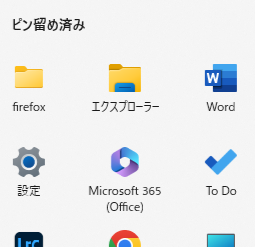
\includegraphics[keepaspectratio, scale=0.8]{image/sc100.pdf}
      \subcaption{100\%}
    \end{minipage} &

    \begin{minipage}[t]{0.45\hsize}
      \centering
      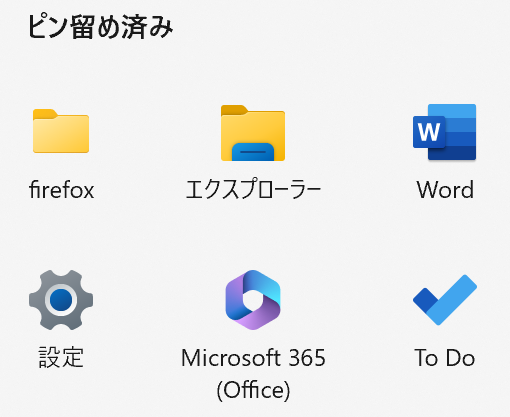
\includegraphics[keepaspectratio, scale=0.4]{image/sc200.pdf}
      \subcaption{200\%}
    \end{minipage} \\

    \begin{minipage}[t]{0.45\hsize}
      \centering
      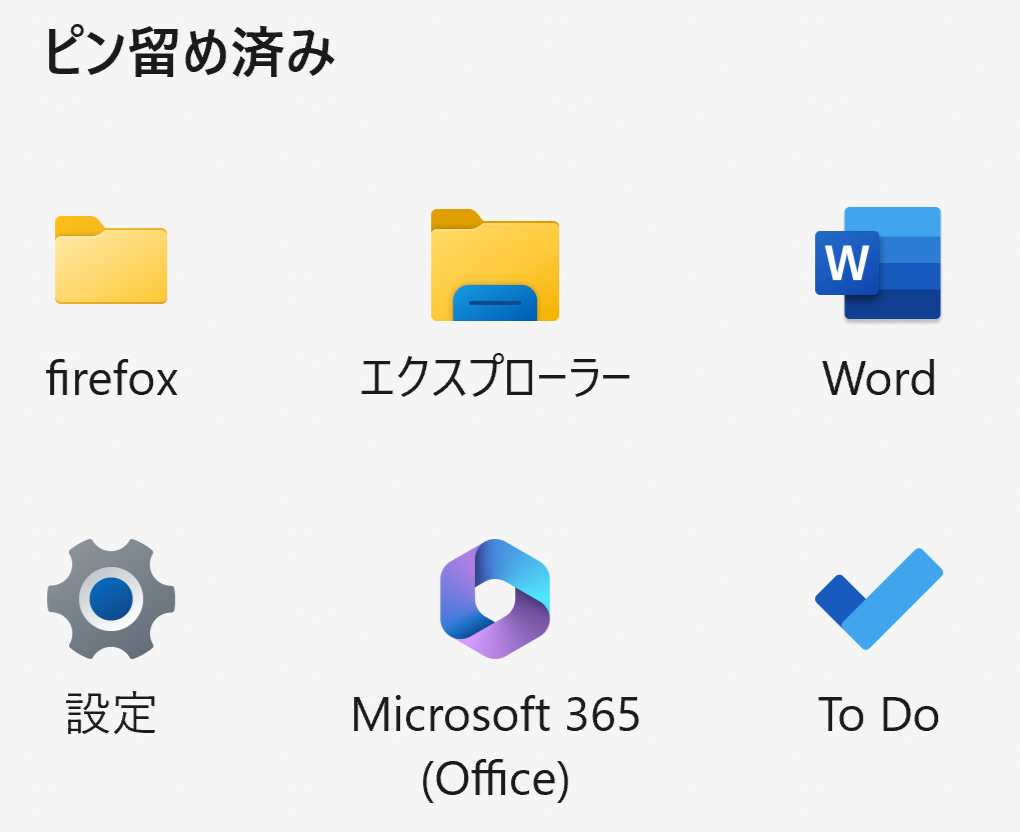
\includegraphics[keepaspectratio, scale=0.2]{image/sc400.pdf}
      \subcaption{400\%}
    \end{minipage}
  \end{tabular}
  \caption{拡大率毎のスクリーンショット} \label{fig:all-screenshot}
\end{figure}